% =====================================================================
%  Primes in Legendre intervals over F_q[t]:
%  an exact explicit-formula algorithm, verification for d <= 10,
%  fluctuations, and an anomaly in characteristic 2
%  DRAFT -- not for distribution
% =====================================================================
\documentclass[11pt,a4paper]{article}

\usepackage[top=28mm,bottom=28mm,left=25mm,right=25mm]{geometry}
\usepackage[T1]{fontenc}
\usepackage{lmodern}
\usepackage{amsmath,amssymb,amsthm,mathtools}
\usepackage{graphicx}
\usepackage{booktabs}
\usepackage[dvipsnames]{xcolor}
\usepackage{enumitem}
\usepackage[colorlinks=true,linkcolor=MidnightBlue,citecolor=MidnightBlue,urlcolor=MidnightBlue]{hyperref}

\newtheorem{theorem}{Theorem}[section]
\newtheorem{lemma}[theorem]{Lemma}
\newtheorem{proposition}[theorem]{Proposition}
\newtheorem{corollary}[theorem]{Corollary}
\newtheorem{conjecture}[theorem]{Conjecture}
\newtheorem{problem}[theorem]{Open problem}
\theoremstyle{definition}
\newtheorem{definition}[theorem]{Definition}
\theoremstyle{remark}
\newtheorem{remark}[theorem]{Remark}

\newcommand{\Fq}{\mathbb{F}_q}
\newcommand{\cI}{\mathcal{I}}
\newcommand{\cG}{\mathcal{G}}
\newcommand{\Nirr}{N_{\mathrm{irr}}}
\newcommand{\Var}{\operatorname{Var}}

\newcommand{\AllQd}{10}
\newcommand{\AllQdNext}{11}
\newcommand{\MaxDtwo}{25}
\newcommand{\MaxDthree}{16}
\newcommand{\MaxDfour}{13}
\newcommand{\MaxDfive}{11}
\newcommand{\MaxDseven}{10}
\newcommand{\MaxDeight}{10}
\newcommand{\MaxDnine}{8}
\newcommand{\Uncertified}{the cases $(2,2)$, $(2,3)$, $(2,4)$, $(2,6)$}
\newcommand{\VarRatioOdd}{between 0.96 and 0.99}
\newcommand{\FormFactorDev}{9\%}
\newcommand{\HistCase}{(3,16)}
\newcommand{\HistIntervals}{14{,}348{,}907}
\newcommand{\MaxExcess}{21}
\newcommand{\MaxRootDev}{$1.0\times10^{-4}$}


\title{\textbf{Primes in Legendre intervals over $\Fq[t]$:\\
an exact explicit-formula algorithm, verification for $d\le\AllQd$,\\
and an anomaly in characteristic 2}}
\author{Ruqing Chen\\[3pt]
\small GUT Geoservice Inc., Montr\'eal, Canada\\
\small \texttt{ruqing@hotmail.com}}
\date{October 2026\\[2pt]\small DOI: \href{https://doi.org/10.5281/zenodo.23225896}{10.5281/zenodo.23225896}\quad
Code and data: \url{https://github.com/Ruqing1963/legendre-intervals-explicit-formula}}

\begin{document}
\maketitle

\begin{abstract}
For monic $f\in\Fq[t]$ of degree $d$, the Legendre interval $\cI_f=\{f^2+s:\deg s\le d\}$ is
the analogue of $[n^2,(n+1)^2]$. The Hayes--Weil estimate shows that $\cI_f$ contains an
irreducible polynomial whenever $q\ge d-1$; the range $q\le d-2$ is open. We give an algorithm
that computes the prime count $\Psi(f)=\sum_{P\in\cI_f}\Lambda(P)$ for \emph{all} $q^{d-1}$
intervals of a given $(q,d)$ at once. It evaluates every Hayes $L$-function by a fast
transform over the Hayes group, whose structure we make explicit for every $\Fq$, and runs in
$O(d^2q^{d-1}+d\,\sigma\,q^{d-1})$ operations, where $\sigma$ is the sum of the orders of the cyclic
factors in our decomposition of the group. Carried out in exact modular arithmetic, it proves that every Legendre interval
contains an irreducible polynomial for every prime power $q$ when $d\le\AllQd$, and for $q=2$
with $d\le\MaxDtwo$, $q=3$ with $d\le\MaxDthree$, $q=4$ with $d\le\MaxDfour$ and $q=5$ with
$d\le\MaxDfive$. For odd $q$ the fluctuations of $\Psi$ across intervals follow the
Keating--Rudnick variance $(d-2)q^{d+1}$ and a Gaussian law already for $q=3$, and the
form factor of the $L$-functions matches the circular unitary ensemble up to an explicit
arithmetic diagonal term. In characteristic $2$ the Legendre intervals form the subgroup of
squares, every element has the shape $h^2+tb^2$, and the variance of $\Psi$ over them differs
from the full-group value, which does follow $d-2$, by factors between $0.33$ and \MaxExcess.
We show that this discrepancy is carried entirely by correlations between $L$-functions twisted by
quadratic characters, and state its explanation as an open problem.
\end{abstract}

\tableofcontents
\bigskip

% =====================================================================
\section{Introduction}
% =====================================================================

Legendre's conjecture asserts that there is a prime between consecutive squares. Its function
field analogue concerns the \emph{Legendre interval}
\[
 \cI_f=\{f^2+s:\ s\in\Fq[t],\ \deg s\le d\},\qquad f\in\Fq[t]\text{ monic of degree }d,
\]
the set of monic polynomials of degree $2d$ whose coefficients of $t^{2d-1},\dots,t^{d+1}$
agree with those of $f^2$. Write
\[
 \Psi(f)=\sum_{P\in\cI_f}\Lambda(P),\qquad \Nirr(f)=\#\{P\in\cI_f:\ P\text{ irreducible}\},
\]
so that $2d\,\Nirr(f)=\Psi(f)-E(f)$ with $E(f)$ the contribution of proper prime powers.

\paragraph{What is known.} Hayes characters and Weil's theorem give
$|\Psi(f)-q^{d+1}|\le(d-2)(q^d-q)$ in every characteristic \cite{Hayes1965,Hsu1996,Cohen2005,Gao2021};
with a bound for $E(f)$ this shows $\Nirr(f)\ge1$ whenever $q\ge d-1$ \cite{ChenV7}. At $q=d-2$
the main term and the error are of the same size, and for $q\le d-2$, which contains the
genuine analogue ($q$ fixed, $d\to\infty$), no method is known. Earlier computations
\cite{ChenV7} tested every element of every interval and reached $d\le8$ for all $q$.

\paragraph{This paper.}
\begin{enumerate}[label=(\arabic*),nosep]
\item \emph{An exact all-intervals algorithm} (Sections~\ref{sec:group}--\ref{sec:algorithm}).
      The values $\Psi(f)$ for all $q^{d-1}$ classes are obtained from the explicit formula,
      computing every Hayes $L$-function by a transform over the Hayes group. We determine an
      explicit basis of this group for every $\Fq$. Done modulo two primes and recombined, the
      computation is exact.
\item \emph{Verification} (Section~\ref{sec:verification}). Every Legendre interval contains an
      irreducible polynomial for all $q$ when $d\le\AllQd$, and much further for small $q$.
\item \emph{Fluctuations and zeros} (Sections~\ref{sec:fluct}--\ref{sec:zeros}). For odd $q$,
      the variance across intervals agrees with Keating--Rudnick \cite{KR2014} at fixed $q$; the
      form factor of the $L$-functions equals an exact arithmetic diagonal for $n\le d-1$ and the
      circular unitary ensemble (CUE) value beyond.
\item \emph{Characteristic 2} (Section~\ref{sec:char2}). The Legendre intervals are the squares
      of the Hayes group; the variance of their prime counts departs from the prediction by factors
      between $0.33$ and \MaxExcess. We show that the departure is carried by correlations between
      quadratic twists and pose its explanation as an open problem.
\end{enumerate}

% =====================================================================
\section{Setup}\label{sec:setup}
% =====================================================================

Let $\ell=d-1$. For monic $g$ of degree $k$ put $[g]=u^kg(1/u)\bmod u^{\ell+1}$, an element of
\[
 \cG=\cG_\ell=\{1+c_1u+\dots+c_\ell u^\ell\}\quad(\text{multiplication mod }u^{\ell+1}),\qquad|\cG|=q^\ell .
\]
The map $g\mapsto[g]$ is multiplicative and records the $\ell$ coefficients below the leading one.
For $x\in\cG$ let $\Psi(x)=\sum_{\deg P=2d,\,[P]=x}\Lambda(P)$; then $\Psi(f)=\Psi([f^2])=\Psi([f]^2)$.

\begin{lemma}\label{lem:legendre-classes}
The interval $\cI_f$ depends only on $f_{d-1},\dots,f_1$; in particular $\cI_{f+c}=\cI_f$ for $c\in\Fq$.
The map $f\mapsto[f]$ from monic polynomials of degree $d$ to $\cG$ is surjective and $q$-to-one, and
$\cI_f$ is the class $[f]^2$. Hence the Legendre intervals are exactly the classes in
$\cG^2=\{x^2:x\in\cG\}$, distinct intervals being distinct classes. If $q$ is odd, $\cG^2=\cG$.
\end{lemma}

\begin{proof}
For $c\in\Fq$, $(f+c)^2-f^2=2cf+c^2$ has degree $\le d$, so $\cI_{f+c}=\cI_f$. The class $[f]$ records
exactly $f_{d-1},\dots,f_1$, which can be chosen freely; this gives surjectivity and the fibres of size $q$
(the choice of $f_0$). Since $[\cdot]$ is multiplicative, $[f^2]=[f]^2$, and $\cI_f$ is by definition the set of
monic $P$ of degree $2d$ with $[P]=[f^2]$. Squaring is a bijection on the finite $p$-group $\cG$ when $p$ is odd.
\end{proof}

For a character $\chi$ of $\cG$ and $n\ge1$ put $\psi_n(\chi)=\sum_{\deg g=n}\Lambda(g)\chi([g])$ and
$c_k(\chi)=\sum_{\deg g=k}\chi([g])$. For $\chi\ne1$, $L(z,\chi)=\sum_kc_k(\chi)z^k$ is a polynomial of
degree $\le\ell-1$ whose inverse roots have absolute value $q^{1/2}$ (Proposition~\ref{prop:conductor}; \cite{Hayes1965,KR2014}),
and $z\,L'(z,\chi)/L(z,\chi)=\sum_n\psi_n(\chi)z^n$. Comparing coefficients gives Newton's recursion
\begin{equation}\label{eq:newton}
 \psi_n(\chi)=n\,c_n(\chi)-\sum_{k=1}^{n-1}\psi_k(\chi)\,c_{n-k}(\chi),\qquad c_n=0\ (n\ge\ell),
\end{equation}
which involves no division. By orthogonality, for every $x\in\cG$,
\begin{equation}\label{eq:explicit}
 \Psi(x)=q^{-\ell}\sum_{\chi}\overline{\chi(x)}\,\psi_{2d}(\chi),\qquad \psi_{2d}(1)=q^{2d}.
\end{equation}

% =====================================================================
\section{The structure of the Hayes group}\label{sec:group}
% =====================================================================

Let $q=p^k$ and let $\omega_0,\dots,\omega_{k-1}$ be a basis of $\Fq$ over $\mathbb F_p$. For $j\ge1$
with $p\nmid j$ let $s_j$ be the least integer with $jp^{s_j}>\ell$.

\begin{proposition}\label{prop:basis}
$\cG_\ell$ is the internal direct product of the cyclic groups generated by $1+\omega_iu^j$,
$p\nmid j\le\ell$, $0\le i<k$, and $1+\omega_iu^j$ has order $p^{s_j}$. In particular
$\cG_\ell\cong\prod_{p\nmid j\le\ell}(\mathbb Z/p^{s_j})^k$.
\end{proposition}

\begin{proof}
In characteristic $p$, $(1+\omega u^j)^{p^s}=1+\omega^{p^s}u^{jp^s}$, which is $1$ modulo
$u^{\ell+1}$ exactly when $jp^s>\ell$; this gives the orders. The orders multiply to
$\prod_jq^{s_j}=q^{\#\{(j,s):\,jp^s\le\ell\}}=q^\ell$, because every $m\le\ell$ is uniquely $jp^s$
with $p\nmid j$. It remains to show that the elements generate. Let $x=1+c_mu^m+O(u^{m+1})$ with
$c_m\ne0$, write $m=jp^a$, and expand $c_m^{p^{-a}}=\sum_ie_i\omega_i$ with $e_i\in\mathbb F_p$. Then
$\prod_i(1+\omega_iu^j)^{e_ip^a}=1+\sum_ie_i\omega_i^{p^a}u^m+O(u^{m+1})=1+c_mu^m+O(u^{m+1})$, so
dividing $x$ by this product raises the order of vanishing of $x-1$. Induction on $m$ expresses
$x$ as a product of the proposed generators.
\end{proof}

The proof is an algorithm: it computes the coordinates of $[g]$ (its \emph{discrete logarithm})
in $O(\ell^2p)$ operations in $\Fq$. Characters of $\cG$ are then
$\chi_b(x)=\prod_{(j,i)}\zeta_{p^{s_j}}^{-a_{j,i}(x)b_{j,i}}$, and sums over $\cG$ weighted by
characters become multidimensional discrete Fourier transforms with axis lengths $p^{s_j}$.

% =====================================================================
\section{The algorithm}\label{sec:algorithm}
% =====================================================================

\begin{enumerate}[label=\arabic*.,nosep]
\item For $k=0,\dots,\ell-1$ form the indicator of $\{[g]:\deg g=k\}$ in the coordinates of
      Proposition~\ref{prop:basis} (for $k\le\ell$ distinct $g$ give distinct classes), and transform
      it to obtain $c_k(\chi)$ for all $\chi$.
\item For every $\chi$ run \eqref{eq:newton} up to $n=2d$.
\item Set $\psi_{2d}(1)=q^{2d}$ and invert the transform to obtain $\Psi(x)$ for all $x$ by \eqref{eq:explicit}.
\end{enumerate}
Step~1 costs $\ell$ transforms, step~2 costs $O(d^2)$ per character, step~3 one transform. With
naive transforms along each axis the total is $O(d^2q^\ell+d\,\sigma\,q^\ell)$ operations, where
$\sigma=k\sum_{p\nmid j\le\ell}p^{s_j}$ is the sum of the orders of the $k\cdot\#\{j\le\ell:p\nmid j\}$ cyclic
factors in Proposition~\ref{prop:basis}. Testing every polynomial costs about $q^{2d}$ instead.

\paragraph{Exact arithmetic.}
All quantities in \eqref{eq:newton}--\eqref{eq:explicit} lie in $\mathbb Z[\zeta][1/q]$, where $\zeta$ is a
primitive $p^S$-th root of unity and $p^S=\max_jp^{s_j}$. For a prime $M\equiv1\pmod{p^S}$, $M\ne p$,
choose $z\in\mathbb F_M$ of order $p^S$; the ring map $\zeta\mapsto z$ turns
\eqref{eq:newton}--\eqref{eq:explicit} into identities in $\mathbb F_M$. Running the algorithm in $\mathbb F_M$
therefore returns $\Psi(x)\bmod M$ exactly. Since $0\le\Psi(x)\le 2d\,q^{d+1}$, two primes
$M_1,M_2<2^{31}$ with $M_1M_2>2dq^{d+1}$ determine $\Psi(x)$ by the Chinese remainder theorem.
All products fit in 64-bit integers.

\paragraph{Checks.} A floating-point version (fast Fourier transforms) is used for exploration.
The exact and floating-point results agree on every class tested; both agree with brute-force counts
for all $11{,}232$ orbit representatives computed in \cite{ChenV7}; and $\sum_x\Psi(x)=q^{2d}$ holds
exactly in every run. For example $q=5$, $d=8$ took one hour by brute force in \cite{ChenV7} and
$0.4$\,s here.

% =====================================================================
\section{Verification}\label{sec:verification}
% =====================================================================

An interval is \emph{certified} if $\Psi(f)>d\,q^a+2q^{\lfloor2d/3\rfloor}$, with $a=1$ for odd $q$
and $a=\lceil(d+1)/2\rceil$ for even $q$; by \cite[Lemma~2.3]{ChenV7} this bound exceeds $E(f)$, so a
certified interval contains an irreducible polynomial.

\begin{remark}[The exponent $a$]
The dominant part of $E(f)$ comes from squares $\pi^2\in\cI_f$ with $\deg\pi=d$, each contributing $d$.
If $q$ is odd, the coefficient of $t^{2d-j}$ in $\pi^2$ is $2\pi_{d-j}$ plus a polynomial in
$\pi_{d-1},\dots,\pi_{d-j+1}$, so the $d-1$ prescribed coefficients determine $\pi_{d-1},\dots,\pi_1$ and at
most $q$ polynomials $\pi$ qualify. If $q$ is even, $\pi^2=\sum_i\pi_i^2t^{2i}$ has no odd-degree terms, so
only the prescribed coefficients in even positions carry information. They determine just
$\lfloor(d-1)/2\rfloor$ coefficients of $\pi$, which leaves up to $q^{\lceil(d+1)/2\rceil}$ candidates.
\end{remark}

\begin{theorem}[computer-assisted]\label{thm:verify}
Every Legendre interval over $\Fq$ contains an irreducible polynomial in each of the following cases:
$q=2$, $d\le\MaxDtwo$; $q=3$, $d\le\MaxDthree$; $q=4$, $d\le\MaxDfour$; $q=5$, $d\le\MaxDfive$;
$q=7$, $d\le\MaxDseven$; $q=8$, $d\le\MaxDeight$; $q=9$, $d\le\MaxDnine$. Consequently the
function field analogue of Legendre's conjecture holds for every prime power $q$ when $d\le\AllQd$.
\end{theorem}

\begin{proof}
For each listed $(q,d)$ the exact algorithm computes $\Psi$ on every Legendre class, and all classes are
certified except some classes in \Uncertified. For these four cases Table~\ref{tab:lowdeg} lists every
Legendre interval with $\Psi(f)$, $E(f)$ and $\Nirr(f)$, obtained by testing every element and enumerating
the prime powers; in each of them $\Nirr(f)\ge1$. For the second statement let $d\le\AllQd$: if $q\ge d-1$
use \cite{ChenV7}; otherwise $q\le d-2\le\AllQd-2$ and $q$ is one of the listed prime powers.
\end{proof}

\begin{table}[ht]
\centering\small
\begin{tabular}{rrlrrrr}
\toprule
$q$ & $d$ & $f$ & $\Psi(f)$ & $E(f)$ & $\Nirr(f)$ & bound \\
\midrule
2 & 2 & $t^{2}$ & 8 & 4 & 1 & 12 \\
\addlinespace
2 & 3 & $t^{3}$ & 16 & 4 & 2 & 20 \\
2 & 3 & $t^{3}+t^{2}$ & 16 & 4 & 2 & 20 \\
\addlinespace
2 & 4 & $t^{4}$ & 24 & 8 & 2 & 40 \\
2 & 4 & $t^{4}+t^{3}$ & 24 & 8 & 2 & 40 \\
\addlinespace
2 & 6 & $t^{6}$ & 160 & 16 & 12 & 128 \\
2 & 6 & $t^{6}+t^{4}$ & 160 & 16 & 12 & 128 \\
2 & 6 & $t^{6}+t^{5}$ & 164 & 20 & 12 & 128 \\
2 & 6 & $t^{6}+t^{5}+t^{4}$ & 60 & 12 & 4 & 128 \\
\bottomrule
\end{tabular}
\caption{All Legendre intervals for the four cases in which some interval is not certified by the bound
(last column). Each row is one interval, given by a representative $f$ (with $f_0=0$). Source:
\texttt{data/low\_degree\_char2.csv}, produced by \texttt{code/low\_degree\_cases.py}.}
\label{tab:lowdeg}
\end{table}

\begin{table}[ht]
\centering\small
\begin{tabular}{rrrrrrr}
\toprule
$q$ & $d$ & intervals & $\min\Psi/q^{d+1}$ & certified & open range & time (s) \\
\midrule
2 & 23 & 2{,}048 & 0.9961 & 2{,}048 & yes & 41.1 \\
2 & 24 & 2{,}048 & 0.9964 & 2{,}048 & yes & 87.7 \\
2 & 25 & 4{,}096 & 0.9983 & 4{,}096 & yes & 184.6 \\
\addlinespace
3 & 14 & 1{,}594{,}323 & 0.9958 & 1{,}594{,}323 & yes & 7.6 \\
3 & 15 & 4{,}782{,}969 & 0.9971 & 4{,}782{,}969 & yes & 25.1 \\
3 & 16 & 14{,}348{,}907 & 0.9982 & 14{,}348{,}907 & yes & 81.7 \\
\addlinespace
4 & 11 & 1{,}024 & 0.9981 & 1{,}024 & yes & 2.6 \\
4 & 12 & 1{,}024 & 0.9968 & 1{,}024 & yes & 11.8 \\
4 & 13 & 4{,}096 & 0.9995 & 4{,}096 & yes & 53.7 \\
\addlinespace
5 & 9 & 390{,}625 & 0.9961 & 390{,}625 & yes & 1.1 \\
5 & 10 & 1{,}953{,}125 & 0.9977 & 1{,}953{,}125 & yes & 5.8 \\
5 & 11 & 9{,}765{,}625 & 0.9991 & 9{,}765{,}625 & yes & 34.1 \\
\addlinespace
7 & 8 & 823{,}543 & 0.9982 & 823{,}543 & no & 3.4 \\
7 & 9 & 5{,}764{,}801 & 0.9993 & 5{,}764{,}801 & yes & 26.7 \\
7 & 10 & 40{,}353{,}607 & 0.9997 & 40{,}353{,}607 & yes & 212.4 \\
\addlinespace
8 & 8 & 512 & 0.9963 & 512 & no & 2.5 \\
8 & 9 & 4{,}096 & 0.9993 & 4{,}096 & no & 34.1 \\
8 & 10 & 4{,}096 & 0.9999 & 4{,}096 & yes & 338.6 \\
\addlinespace
9 & 6 & 59{,}049 & 0.9889 & 59{,}049 & no & 0.1 \\
9 & 7 & 531{,}441 & 0.9987 & 531{,}441 & no & 0.6 \\
9 & 8 & 4{,}782{,}969 & 0.9994 & 4{,}782{,}969 & no & 6.0 \\
\bottomrule
\end{tabular}
\caption{Exact verification. ``Intervals'' is the number of Legendre classes; the ratio is
$\min_f\Psi(f)/q^{d+1}$; times are wall-clock for the exact computation (two primes).
Only the largest $d$ for each $q$ and the cases with $q\le d-2$ near the boundary are shown;
all cases are in \texttt{data/exact\_scan.csv}.}
\label{tab:verify}
\end{table}

The case $d=\AllQdNext$ would require $q=7$, $8$ and $9$ with $d=\AllQdNext$, that is up to
$9^{\AllQd}\approx3.5\times10^9$ classes, beyond the memory used here.

% =====================================================================
\section{Fluctuations across intervals}\label{sec:fluct}
% =====================================================================

For odd $q$ every class is a Legendre interval (Lemma~\ref{lem:legendre-classes}), so the
distribution of $\Psi$ over Legendre intervals is the distribution over all $q^{d-1}$ classes.
Keating and Rudnick \cite{KR2014} proved $\Var\Psi\sim(d-2)q^{d+1}$ as $q\to\infty$ (for $d\ge4$).

\begin{figure}[ht]
\centering
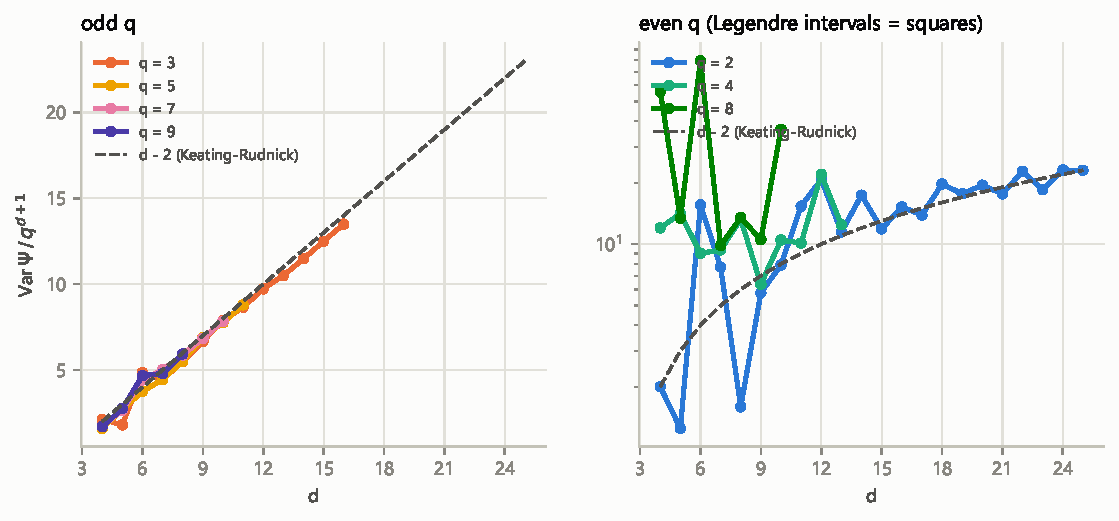
\includegraphics[width=\linewidth]{figures/p2_variance.pdf}
\caption{$\Var_f\Psi(f)/q^{d+1}$ (mean square deviation from $q^{d+1}$) over all Legendre intervals.
Left: odd $q$, against the Keating--Rudnick limit $d-2$. Right: even $q$, where the prediction fails.}
\label{fig:var}
\end{figure}

\begin{figure}[ht]
\centering
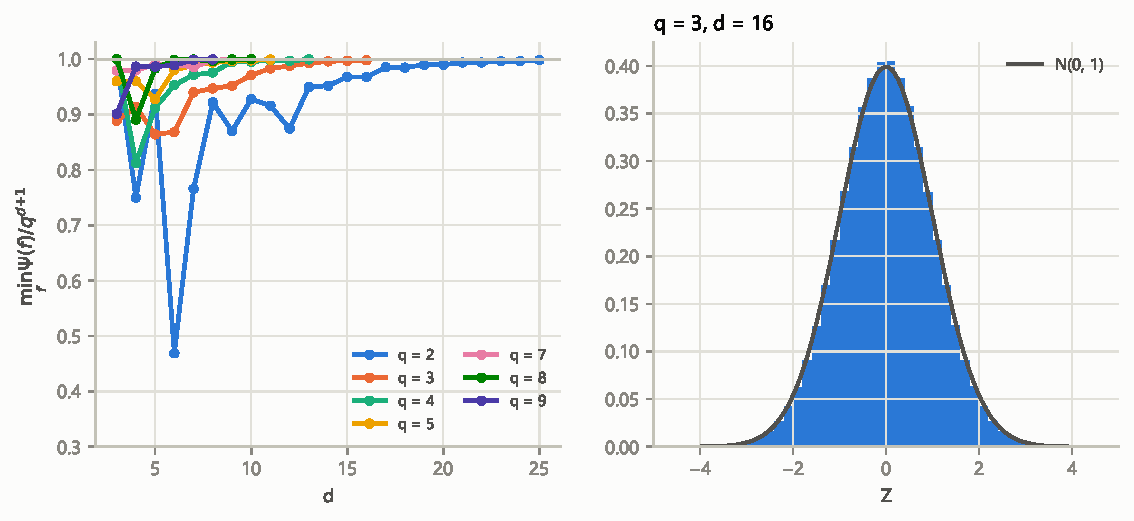
\includegraphics[width=\linewidth]{figures/p2_minratio_hist.pdf}
\caption{Left: $\min_f\Psi(f)/q^{d+1}$ against $d$. Right: the distribution of
$Z=(\Psi-q^{d+1})/\sqrt{(d-2)q^{d+1}}$ over the $\HistIntervals$ intervals with $(q,d)=\HistCase$,
against the standard normal density.}
\label{fig:min}
\end{figure}

For odd $q$ the ratio $\Var\Psi/((d-2)q^{d+1})$ is \VarRatioOdd\ for the largest computed $d$ of each
$q$ (Figure~\ref{fig:var}), and $Z$ is close to Gaussian (Figure~\ref{fig:min}). The minimum of $\Psi$
approaches $q^{d+1}$ as $d$ grows, as the Gaussian heuristic of \cite{ChenV7} predicts.

% =====================================================================
\section{The zeros}\label{sec:zeros}
% =====================================================================

\begin{proposition}\label{prop:conductor}
For $\chi\ne1$ let $m(\chi)$ be the least $m$ such that $\chi$ is trivial on $\{x\in\cG:x\equiv1\bmod u^m\}$,
so $2\le m(\chi)\le\ell+1$. Then $L(z,\chi)$ has degree exactly $m(\chi)-2$, and all its inverse roots have
absolute value $q^{1/2}$. Exactly $q^{m-1}-q^{m-2}$ characters have $m(\chi)=m$.
\end{proposition}

\begin{proof}
Write $\hat g(u)=u^{\deg g}g(1/u)$. For monic $g$ of degree $k$, $\hat g$ runs over the polynomials $h$ with
$h(0)=1$ and $\deg h\le k$, bijectively, and $[g]=h\bmod u^{\ell+1}$. Hence
\[
 L(z,\chi)=\sum_{h(0)=1}\chi(h)\,z^{\deg h}\sum_{k\ge\deg h}z^k=\frac{L_{\mathrm{D}}(z,\chi)}{1-z},\qquad
 L_{\mathrm D}(z,\chi)=\sum_{h(0)=1}\chi(h)\,z^{\deg h},
\]
where $L_{\mathrm D}(z,\chi)$ is the Dirichlet $L$-function of $\chi$ viewed as an
even character modulo $u^{\ell+1}$ in $\Fq[u]$ (scaling by the constant term identifies polynomials with $h(0)=1$
with monic polynomials prime to $u$, and $\chi$ is trivial on constants). The character is induced from a
primitive even character modulo $u^{m(\chi)}$, and since $u$ is the only prime dividing either modulus,
$L_{\mathrm D}$ is unchanged by passing to the primitive character. For a primitive even character modulo a
polynomial of degree $m\ge2$, $L_{\mathrm D}(z)=(1-z)P(z)$ with $P$ of degree $m-2$ whose inverse roots all
have absolute value $q^{1/2}$ (Weil; see \cite[Ch.~4]{Rosen2002} and \cite[\S4]{KR2014}). So
$L(z,\chi)=P(z)$. The characters with $m(\chi)\le m$ are those of the quotient $\cG_{m-1}$, which has $q^{m-1}$
elements.
\end{proof}

The computed $L$-functions confirm this exactly: in every case of Table~\ref{tab:zeros} the number of
characters of each conductor $u^m$ is $q^{m-1}-q^{m-2}$, the coefficient $c_{m-2}(\chi)$ is nonzero and all
higher ones vanish. The inverse roots were then computed numerically from the exact-degree polynomials. Their
absolute values are $\sqrt q$ to within $10^{-6}$ relative error, except for roots of multiplicity greater
than one, where floating-point root finding is less accurate; the largest deviation is \MaxRootDev. The only
such case with a deviation above $10^{-5}$ is one quadratic character for $(q,d)=(4,10)$, whose $L$-function is
$(1+2z)^4(1-2z+4z^2)^2$.

Let $F(n)=(q^\ell-1)^{-1}\sum_{\chi\ne1}|\psi_n(\chi)|^2/q^n$. Writing the inverse roots as $\sqrt q\,e^{i\theta}$,
$F(n)$ is the average of $|\sum e^{in\theta}|^2$; for $N\times N$ CUE matrices this average is $\min(n,N)$.

\begin{proposition}\label{prop:diagonal}
For $1\le n\le\ell$,
\[
 F(n)=\frac{q^\ell S_n-q^{2n}}{(q^\ell-1)\,q^n},\qquad S_n=\sum_{\deg g=n}\Lambda(g)^2=\sum_{e\mid n}e^2I_e(q),
\]
where $I_e(q)$ is the number of monic irreducible polynomials of degree $e$. In particular
$F(n)=n+O(n^2q^{-n/2})+O(q^{n-\ell})$, and $F(2)=2-1/q+O(q^{2-\ell})$.
\end{proposition}

\begin{proof}
By Parseval, $\sum_\chi|\psi_n(\chi)|^2=q^\ell\sum_{x}\bigl(\sum_{\deg g=n,[g]=x}\Lambda(g)\bigr)^2$. For monic
$g=t^n+g_{n-1}t^{n-1}+\dots+g_0$ we have $[g]=1+g_{n-1}u+\dots+g_0u^n$ modulo $u^{\ell+1}$. If $n\le\ell$ no
coefficient is lost in the truncation, so $g\mapsto[g]$ is injective on monic polynomials of degree $n$: exactly
$q^n$ classes contain one such polynomial and the other $q^\ell-q^n$ contain none. The inner sum therefore has
at most one term and the total is $q^\ell S_n$. Remove the trivial character, $|\psi_n(1)|^2=q^{2n}$.
\end{proof}

The computed $F(n)$ agree with Proposition~\ref{prop:diagonal} to $10^{-14}$. For $n>\ell$ there is no such
formula; there $F(n)$ is the variance of prime counts in classes of degree-$n$ polynomials, and it stays
within \FormFactorDev\ of the CUE value $\ell-1$ (Figure~\ref{fig:zeros}). The nearest-neighbour
spacings of the eigenangles agree with CUE$(d-2)$ to within $0.05$ in density.

\begin{figure}[ht]
\centering
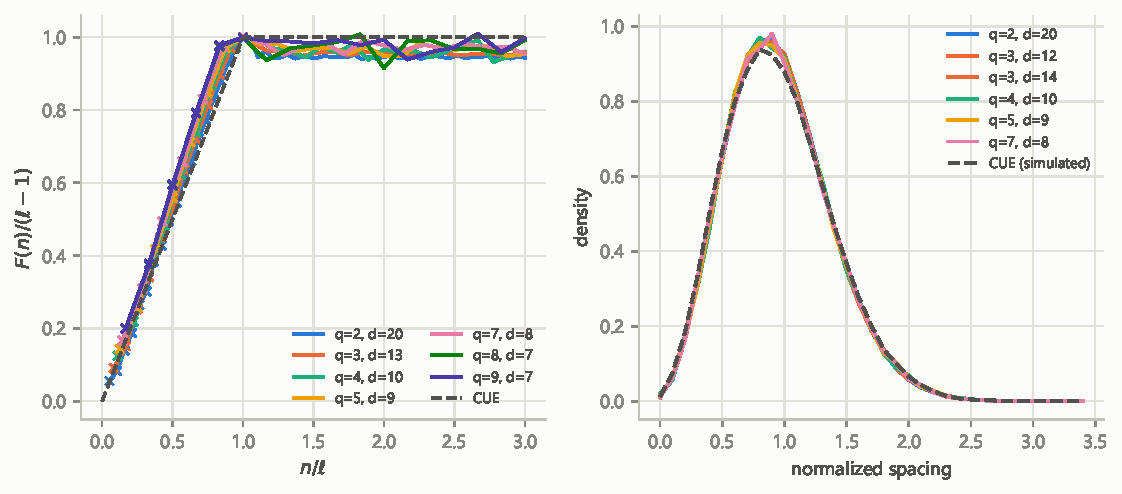
\includegraphics[width=\linewidth]{figures/p2_zeros.pdf}
\caption{Left: the form factor $F(n)/(\ell-1)$ against $n/\ell$ for several $(q,d)$, with the CUE value
$\min(n,\ell-1)/(\ell-1)$ and the exact diagonal of Proposition~\ref{prop:diagonal} (crosses). Right:
nearest-neighbour spacing densities against CUE.}
\label{fig:zeros}
\end{figure}

\begin{table}[ht]
\centering\small
\begin{tabular}{rrrrr}
\toprule
$q$ & $d$ & characters & generic & roots off $|\omega|=\sqrt q$ \\
\midrule
2 & 20 & 400{,}000 & 0.5009 & 0 \\
3 & 12 & 177{,}146 & 0.6667 & 0 \\
3 & 14 & 400{,}000 & 0.6672 & 0 \\
4 & 10 & 262{,}143 & 0.7500 & 2 \\
5 & 9 & 390{,}624 & 0.8000 & 0 \\
7 & 8 & 400{,}000 & 0.8576 & 0 \\
\bottomrule
\end{tabular}
\caption{Zeros of the Hayes $L$-functions for the listed $(q,d)$ (all characters, or a random sample of
$400{,}000$). ``Generic'' is the proportion of characters with conductor $u^{\ell+1}$, i.e.\ with the maximal
degree $d-2$; the exact proportion is $(q^\ell-q^{\ell-1})/(q^\ell-1)$. The last column is the largest relative
deviation of $|\omega|$ from $\sqrt q$ over all computed inverse roots.}
\label{tab:zeros}
\end{table}

% =====================================================================
\section{Characteristic 2}\label{sec:char2}
% =====================================================================

\subsection{Structure}
Let $q$ be even. By Lemma~\ref{lem:legendre-classes} the Legendre intervals form the subgroup $\cG^2$ of
index $2^{k\cdot\#\{j\le\ell\ \mathrm{odd}\}}$. Their elements have a special form.

\begin{proposition}\label{prop:char2}
Let $q$ be even and $f$ monic of degree $d$. Every $P\in\cI_f$ can be written uniquely as
\[
 P=h^2+t\,b^2,\qquad h=f+a,\ \deg a\le\lfloor d/2\rfloor,\ \deg b\le\lfloor(d-1)/2\rfloor .
\]
Then $P'=b^2$, and $P$ is squarefree if and only if $\gcd(h,b)=1$.
\end{proposition}

\begin{proof}
Write $s=P-f^2$ as $a(t)^2+t\,b(t)^2$ by separating even and odd powers (every element of $\Fq$ is a
square); then $f^2+s=(f+a)^2+tb^2$ because squaring is additive. Differentiating, $P'=b^2$. If $\pi^2\mid P$
for an irreducible $\pi$, then $\pi\mid P'=b^2$, so $\pi\mid b$ and $\pi\mid h^2$, so $\pi\mid h$. Conversely if
$\pi\mid h$ and $\pi\mid b$ then $\pi^2$ divides both $h^2$ and $tb^2$. If $b=0$ then $P=h^2$ is not squarefree,
and $\gcd(h,0)=h$ is nonconstant.
\end{proof}

Thus a Legendre interval in characteristic $2$ is a union, over the $q^{\lfloor(d+1)/2\rfloor}$ values of $b$,
of the values of the quadratic polynomial $X^2+tb^2$ on a short interval of $X$ around $f$. Counting its
primes is closer to a Bateman--Horn problem for quadratic polynomials than to counting primes in an interval.

\subsection{The anomaly}

\begin{table}[ht]
\centering\small
\begin{tabular}{rrrrrrrrr}
\toprule
$q$ & $d$ & mean & Var (all) & Var (Legendre) & ratio & excess & $\Sigma\rho$, order 2 & $\Sigma\rho$, other \\
\midrule
2 & 4 & 0.7500 & 1.50 & 2.00 & 1.33 & 1.33 & -0.33 & +0.67 \\
2 & 5 & 1.0625 & 1.17 & 1.25 & 1.07 & 1.07 & -0.36 & +0.43 \\
2 & 6 & 1.0625 & 5.76 & 15.56 & 2.70 & 2.70 & +0.53 & +1.18 \\
2 & 7 & 1.0469 & 3.88 & 7.72 & 1.99 & 1.99 & +0.24 & +0.74 \\
2 & 8 & 0.9688 & 4.88 & 1.59 & 0.33 & 0.33 & +0.21 & -0.88 \\
2 & 9 & 0.9805 & 7.10 & 5.77 & 0.81 & 0.81 & -0.40 & +0.21 \\
2 & 10 & 1.0273 & 7.19 & 7.91 & 1.10 & 1.10 & +0.24 & -0.14 \\
2 & 11 & 0.9985 & 8.57 & 15.35 & 1.79 & 1.79 & +0.21 & +0.58 \\
2 & 12 & 0.9839 & 9.75 & 20.74 & 2.13 & 2.13 & +0.13 & +1.00 \\
2 & 13 & 1.0044 & 10.10 & 11.47 & 1.14 & 1.14 & -0.09 & +0.23 \\
2 & 14 & 0.9995 & 11.30 & 17.37 & 1.54 & 1.54 & +0.24 & +0.29 \\
2 & 15 & 0.9995 & 12.10 & 11.86 & 0.98 & 0.98 & +0.02 & -0.04 \\
2 & 16 & 0.9983 & 13.19 & 15.22 & 1.15 & 1.15 & +0.04 & +0.12 \\
\addlinespace
4 & 4 & 1.0000 & 2.25 & 12.00 & 5.33 & 5.33 & +0.33 & +4.00 \\
4 & 5 & 1.0117 & 2.60 & 14.11 & 5.43 & 5.43 & +0.83 & +3.60 \\
4 & 6 & 0.9883 & 3.70 & 9.01 & 2.44 & 2.44 & +1.34 & +0.09 \\
4 & 7 & 1.0037 & 5.23 & 9.36 & 1.79 & 1.79 & +0.42 & +0.36 \\
4 & 8 & 1.0000 & 5.88 & 13.25 & 2.25 & 2.25 & +0.07 & +1.18 \\
4 & 9 & 0.9999 & 6.79 & 6.36 & 0.94 & 0.94 & -0.02 & -0.04 \\
\addlinespace
8 & 4 & 0.9727 & 2.62 & 56.00 & 21.33 & 21.33 & +1.67 & +18.67 \\
8 & 5 & 1.0017 & 3.11 & 13.41 & 4.31 & 4.31 & +0.28 & +3.03 \\
8 & 6 & 1.0017 & 4.75 & 79.09 & 16.66 & 16.66 & +2.21 & +13.45 \\
8 & 7 & 1.0002 & 4.96 & 9.85 & 1.99 & 1.99 & +0.00 & +0.98 \\
\bottomrule
\end{tabular}
\caption{Characteristic 2. The two variance columns are the mean of $(\Psi-q^{d+1})^2/q^{d+1}$ over all
classes of $\cG$ and over the Legendre intervals $\cG^2$; ``mean'' is the mean of $\Psi/q^{d+1}$ over $\cG^2$;
``ratio'' is the quotient of the two variances, and ``excess'' is $1+\sum_{\varepsilon\ne1}\rho(\varepsilon)$ from
\eqref{eq:rho}. Source: \texttt{data/char2\_variance.csv}.}
\label{tab:char2}
\end{table}

Table~\ref{tab:char2} compares the variance of $\Psi$ over all classes of $\cG$ with the variance over the
Legendre intervals $\cG^2$. Over all classes the variance follows $d-2$ for even $q$ just as for odd $q$,
and the form factor over all characters matches CUE for $q=2,4,8$ (Figure~\ref{fig:zeros}). Over $\cG^2$
the variance differs from it by a factor that ranges from about $0.33$ to \MaxExcess, while the mean
stays close to $q^{d+1}$. The anomaly is therefore a property of the subfamily $\cG^2$, not of the
$L$-functions as a whole.

By Parseval on $\cG^2$, $\Var_{\cG^2}\Psi$ is governed by the sums $\sum_{\varepsilon}\psi_{2d}(\chi\varepsilon)$ over
characters $\varepsilon$ trivial on $\cG^2$, i.e.\ the characters of order $\le2$. If $\psi_{2d}(\chi)$ and
$\psi_{2d}(\chi\varepsilon)$ were uncorrelated, the variance would equal the full-group value. Define
\begin{equation}\label{eq:rho}
 \rho(\varepsilon)=\frac{\operatorname{Re}\sum_{\chi\ne1}\psi_{2d}(\chi)\overline{\psi_{2d}(\chi\varepsilon)}}{\sum_{\chi\ne1}|\psi_{2d}(\chi)|^2}.
\end{equation}
The ratio of the two variances is $1+\sum_{\varepsilon\ne1}\rho(\varepsilon)$ up to the trivial-character terms, and
in every case of Table~\ref{tab:char2} the two columns coincide to four decimals. The whole anomaly is
thus carried by correlations between quadratic twists.

\paragraph{Where the correlations sit.}
Let $q$ be even. By Proposition~\ref{prop:basis}, $\cG\cong\prod_{j\le\ell\text{ odd}}(\mathbb Z/2^{s_j})^k$, and
$\cG^2$ is the subgroup of elements whose coordinates are all even. Hence $\cG/\cG^2\cong(\mathbb Z/2)^{k\,m}$
with $m=\#\{j\le\ell\text{ odd}\}$, and the characters trivial on $\cG^2$ are
$\varepsilon(x)=(-1)^{\sum_{(j,i)}e_{j,i}a_{j,i}(x)}$ with $e_{j,i}\in\{0,1\}$. The coordinates with $j>\ell/2$
are exactly those with $s_j=1$, that is, the generators $1+\omega_iu^j$ of order $2$; there are
$k\cdot\#\{j\text{ odd}:\ \ell/2<j\le\ell\}$ of them. One might expect the twists supported on these
coordinates to carry the effect, but they do not: Table~\ref{tab:char2} splits $\sum_{\varepsilon\ne1}\rho(\varepsilon)$ into
the part from $\varepsilon$ with $e_{j,i}=0$ for all $j<\ell/2$ and the rest, and in most cases the rest dominates
(for example $1.67$ against $18.67$ for $(q,d)=(8,4)$). The correlations are spread over many quadratic twists,
and we have no structural description of which twists correlate.

Two natural explanations fail. On fixed-$b$ slices, $\mu(h^2+tb^2)$ is neither of the form
$\pm(-1)^{L(a)}$ with $L$ affine over $\mathbb F_2$ in the coefficients of $a$, nor a function of
$h\bmod b$ alone (tested for $d=8,10,12$, $q=2$).

The natural framework is the parity of the number of prime factors. In odd characteristic it is given by
Pellet's formula through the discriminant; in characteristic $2$ Pellet's formula fails, and Carmon
\cite{Carmon2015} replaced the discriminant by Berlekamp's discriminant to prove the function field Chowla
conjecture in characteristic $2$ in the limit $q\to\infty$. For $P=h^2+tb^2$ the derivative $P'=b^2$ depends
only on $b$, which is the situation in which Sawin and Shusterman \cite{SawinShusterman2022} turn the
M\"obius function into a Dirichlet character in odd characteristic. Whether an analogue of their mechanism,
through Berlekamp's discriminant, accounts for the correlations is open.

\begin{problem}\label{prob:char2}
Explain the excess variance of $\Psi$ over Legendre intervals in characteristic $2$: determine
$\lim\Var_{\cG^2}\Psi/q^{d+1}$, as $q\to\infty$ through powers of $2$ and as $d\to\infty$, and identify
the mechanism behind the correlations $\rho(\varepsilon)$, presumably through the Berlekamp discriminant
and the form $P=h^2+tb^2$ with $P'=b^2$ \cite{Carmon2015,SawinShusterman2022}.
\end{problem}

\paragraph{Note added in proof.}
In the sequel \cite{Chen2026b}, Problem~\ref{prob:char2} is resolved for $d=4$:
$\Var_{\cG^2}\Psi/q^5=q(q-1)$ and $\Var_{\cG}\Psi/q^5=3-3/q$ are proved for all $q=2^k$
via the quadratic tower $\Fq\subset\mathbb F_{q^2}\subset\mathbb F_{q^4}\subset\mathbb F_{q^8}$,
and the correlations $\rho(\varepsilon)$ are determined ($\rho=1$ on the $q-1$ twists of conductor $u^2$,
$\rho=(q-3)/(3(q-1))$ on all others for odd $k$). For $d=6$ the Legendre profile is shown to take exactly
three values, and exact computations up to $q=32$ ($q=128$ for two of the three governing constants)
establish $\Var_{\cG^2}\Psi/q^7\asymp q^2$, excluding the $q^4$ law one might have expected.

% =====================================================================
\section{Discussion}
% =====================================================================

The explicit formula reduces the verification of the function field Legendre conjecture to a
transform over the Hayes group, and exact modular arithmetic makes the result a proof. The method
reaches every $q$ for $d\le\AllQd$; going further needs memory proportional to $q^{d-1}$, so the next step,
$q=7,8,9$ with $d=11$, needs either a distributed transform or a reduction by symmetry. The substitutions
$t\mapsto\lambda t+b$ and the Frobenius automorphism of $\Fq$ act on classes of degree $2d$ by affine maps of
$\cG$ (an automorphism followed by a translation) and preserve $\Psi$; for $q=9$ this group has order
$2\cdot9\cdot8=144$. A transform adapted to this action could reduce the memory by a factor of that order,
but we have not implemented it, and whether it brings $(9,11)$ within reach of one machine is untested.

The data support the conjecture of \cite{ChenV7} that no Legendre interval is ever empty. For odd $q$ the
fluctuations behave as random matrix theory predicts already at $q=3$; in characteristic $2$ they do not,
for a reason that Problem~\ref{prob:char2} asks to explain.

\paragraph{Code and data.} All programs and results are in the repository
\begin{center}\small\url{https://github.com/Ruqing1963/legendre-intervals-explicit-formula}\end{center}
The files named in the text (\texttt{exact\_scan.csv}, \texttt{char2\_variance.csv},
\texttt{low\_degree\_char2.csv}) are in its \texttt{data} directory. This paper is archived as
\href{https://doi.org/10.5281/zenodo.23225896}{doi:10.5281/zenodo.23225896}.

\begin{thebibliography}{99}
\bibitem{Carmon2015} D.~Carmon, The autocorrelation of the M\"obius function and Chowla's conjecture
 for the rational function field in characteristic 2, \textit{Philos.\ Trans.\ Roy.\ Soc.\ A} \textbf{373} (2015). arXiv:1409.3694.
\bibitem{Chen2026b} R.~Chen, Prime polynomials in Legendre intervals over $\mathbb F_{2^k}[t]$, II:
 exact variances via quadratic towers and supersingular Artin--Schreier curves, preprint (2026),
 DOI 10.5281/zenodo.23224897.
\bibitem{ChenV7} R.~Chen, Legendre's conjecture in function fields: the classical range, full monodromy,
 and the open range $q\le d-2$ (v7), Zenodo, 2026. \url{https://doi.org/10.5281/zenodo.23185896}
\bibitem{Cohen2005} S.\,D.~Cohen, Explicit theorems on generator polynomials,
 \textit{Finite Fields Appl.}\ \textbf{11} (2005), 337--357.
\bibitem{Gao2021} Z.~Gao, Improved error bounds for the number of irreducible polynomials and
 self-reciprocal irreducible monic polynomials with prescribed coefficients over a finite field, arXiv:2109.14154.
\bibitem{Hayes1965} D.\,R.~Hayes, The distribution of irreducibles in $GF[q,x]$,
 \textit{Trans.\ Amer.\ Math.\ Soc.}\ \textbf{117} (1965), 101--127.
\bibitem{Hsu1996} C.\,N.~Hsu, The distribution of irreducible polynomials in $\mathbb F_q[t]$,
 \textit{J.\ Number Theory} \textbf{61} (1996), 85--96.
\bibitem{KR2014} J.\,P.~Keating, Z.~Rudnick, The variance of the number of prime polynomials in short
 intervals and in residue classes, \textit{Int.\ Math.\ Res.\ Not.}\ 2014, 259--288.
\bibitem{Rosen2002} M.~Rosen, \textit{Number Theory in Function Fields}, Graduate Texts in Mathematics 210,
 Springer, 2002.
\bibitem{SawinShusterman2022} W.~Sawin, M.~Shusterman, On the Chowla and twin primes conjectures over
 $\mathbb F_q[T]$, \textit{Ann.\ of Math.}\ \textbf{196} (2022). arXiv:1808.04001.
\end{thebibliography}
\end{document}
